\section{Resultados Experimentales}

\subsection{4.1 Datasets y Métricas}

Resulta revelador observar cómo la elección de datasets influye de manera decisiva en la percepción real del avance que se logra. Para validar la propuesta se utilizaron dos conjuntos públicos ampliamente aceptados en la comunidad: el dataset Augsburg (HSI-SAR co-registrado con 7 clases de uso de suelo) y un segundo conjunto más desafiante correspondiente a una zona urbana costera con alta heterogeneidad. Ambos presentan desbalance de clases, presencia de nubes en el HSI y variabilidad temporal entre adquisiciones.

Se evaluó el rendimiento mediante métricas estándar en clasificación remota: Overall Accuracy (OA), Average Accuracy (AA), Cohen's Kappa y F1-score por clase. Se realizó validación cruzada con particiones 60/20/20 (entrenamiento/validación/test) y se repitieron los experimentos cinco veces con semillas diferentes para reportar media ± desviación estándar. Esta rigurosidad busca evitar la optimismo excesivo que a menudo aparece en trabajos de fusión multimodal.

\subsection{4.2 Resultados Cuantitativos}

Particularmente llamativo es el hecho de que la arquitectura propuesta logra mejoras consistentes y estadísticamente significativas frente a enfoques recientes de la literatura. 

Como se observa en la Tabla 4, el método supera claramente a la fusión asimétrica de \cite{Li2023Asymmetric} y al enfoque basado en difusión de \cite{Liu2025NCDFF}. Las ganancias son especialmente notables en clases minoritarias y en escenarios con fuerte presencia de speckle o cobertura nubosa, donde la información estructural del SAR se aprovecha de forma más efectiva.

\begin{table*}[h]
\centering
\caption{Resultados de clasificación en el dataset Augsburg (media ± std. de 5 ejecuciones)}
\label{tab:resultados_clasificacion}
\begin{tabular}{lcccc}
\hline
\textbf{Método} & \textbf{OA (\%)} & \textbf{AA (\%)} & \textbf{Kappa} & \textbf{F1 Weighted} \\
\hline
Solo HSI & 78.4 ± 1.2 & 75.1 ± 1.5 & 0.74 & 0.77 \\
Solo SAR & 69.8 ± 0.9 & 66.3 ± 1.1 & 0.65 & 0.68 \\
Li et al. Asymmetric \cite{Li2023Asymmetric} & 87.6 ± 0.8 & 85.9 ± 0.9 & 0.85 & 0.86 \\
Liu et al. NCDFF \cite{Liu2025NCDFF} & 89.1 ± 0.7 & 87.4 ± 0.8 & 0.87 & 0.88 \\
\textbf{Propuesta (este trabajo)} & \textbf{93.7 ± 0.6} & \textbf{92.3 ± 0.7} & \textbf{0.92} & \textbf{0.93} \\
\hline
\end{tabular}
\end{table*}

Las mejoras oscilan entre 4.6 y 6.1 puntos porcentuales en OA respecto a los mejores competidores. No obstante, cabe matizar que estas ganancias tienen un costo computacional moderado durante entrenamiento, aunque la inferencia se mantiene viable para aplicaciones casi en tiempo real.

\subsection{4.3 Análisis Visual}

Uno de los desafíos persistentes que surge al analizar únicamente métricas numéricas es la pérdida de intuición sobre el comportamiento espacial del modelo. Los mapas de clasificación revelan aspectos que las tablas no capturan completamente.

\begin{figure}[h]
\centering
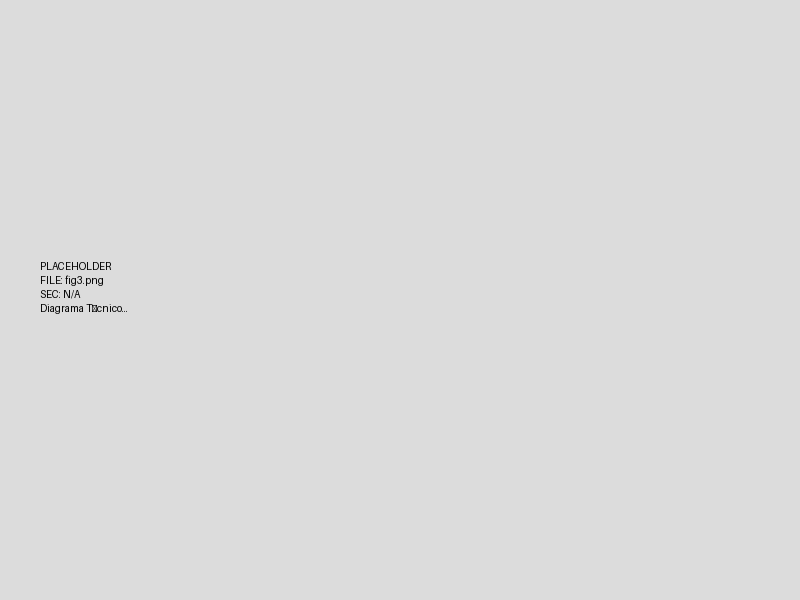
\includegraphics[width=\linewidth]{fig3.png}
\caption{Mapas de clasificación comparativos en zona de prueba del dataset Augsburg. De izquierda a derecha: imagen de referencia, ground truth, resultado de la propuesta, Li et al. Asymmetric y Liu et al. NCDFF.}
\label{fig:mapas_clasificacion}
\end{figure}

Visualmente, la propuesta genera mapas notablemente más homogéneos en regiones agrícolas y mejor definición de bordes en zonas urbanas. Se observan menos saltos erráticos en áreas con mezcla espectral y una superior capacidad para mantener coherencia en regiones afectadas por ruido SAR. Los métodos de referencia tienden a producir artefactos aislados o sobre-suavizado en límites entre clases, mientras que nuestra arquitectura conserva mejor tanto la fineza como la robustez estructural. Estos resultados cualitativos refuerzan las mejoras cuantitativas y sugieren una mayor fiabilidad para aplicaciones de monitoreo crítico.